\DailyTitle{6311 Log (October 11, 2010)}

\DailySection{Goals}

\begin{enumerate}
\item Submit vecbos ntuple jobs
\item Make a to-write list for Z candle
\item Do one round of subtraction and look at remaining noise
\item Try out Hcal DQM GUI on lxplus
\end{enumerate}

\DailySection{Summary List}

\begin{enumerate}
\item Yay
\end{enumerate}

\DailySection{Vecbos ntuple jobs}

Submitted jobs for \texttt{Jet} and \texttt{METFwd} datasets.  Wait until afternoon, if things are looking good then I will submit the \texttt{JetMET} dataset.
This one is a lot larger than the other two newer datasets.

\DailySection{Update errors to $\chi^2$ instead of $error^2$}

Just replace all error calculation parts by $\chi^2$, ie., divide the deviations by the charge of that time slice.  Let's see if the result will be improved.

The linear one seems better!  Shown in figures \ref{Figure_6311HTestStatisticsLinearFit} and \ref{Figure_6311HTestStatisticsLinearFit100}.
The small group of pulses in signal distribution that is smaller than zero needs more attention.  If they were noise, that will be really great.

\begin{figure}
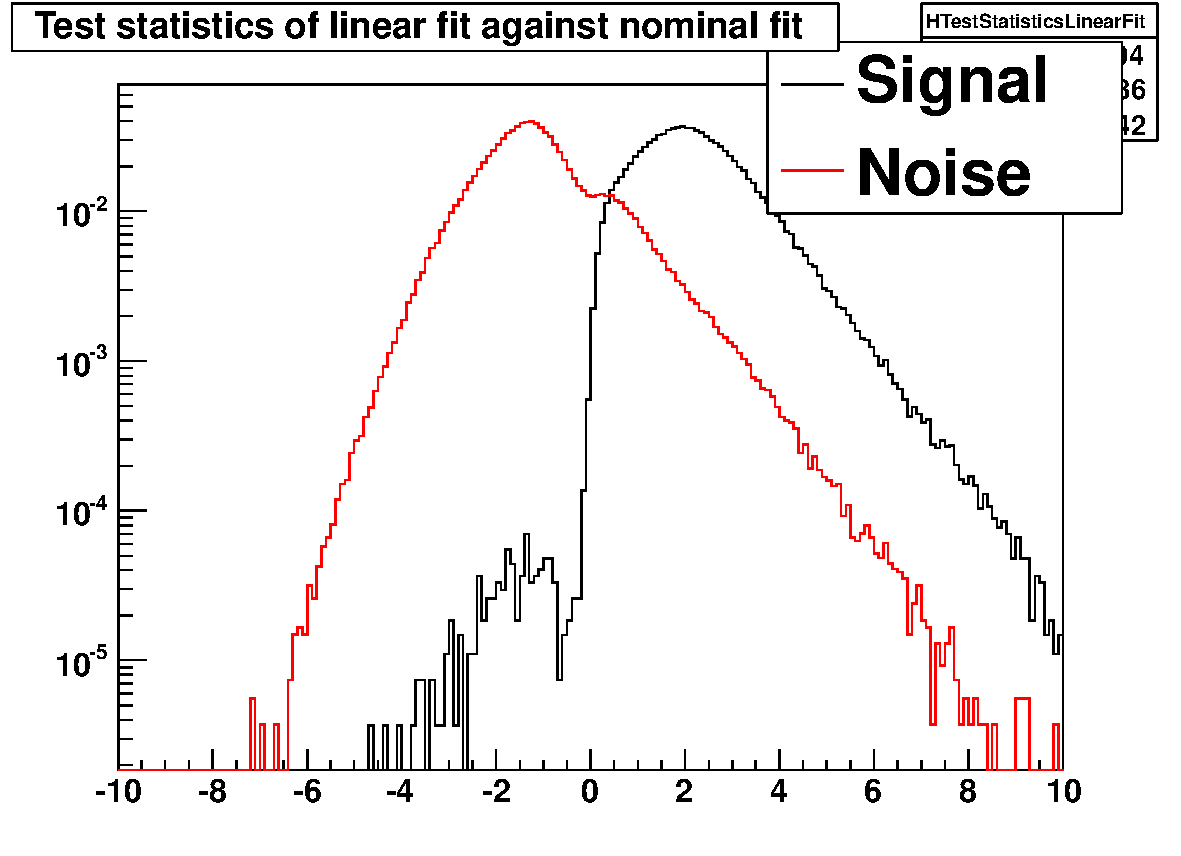
\includegraphics[width=120mm]{DailyLog/6311/6311HTestStatisticsLinearFit.pdf}
\caption{Test statistics on linear fit.}
\label{Figure_6311HTestStatisticsLinearFit}
\end{figure}

\begin{figure}
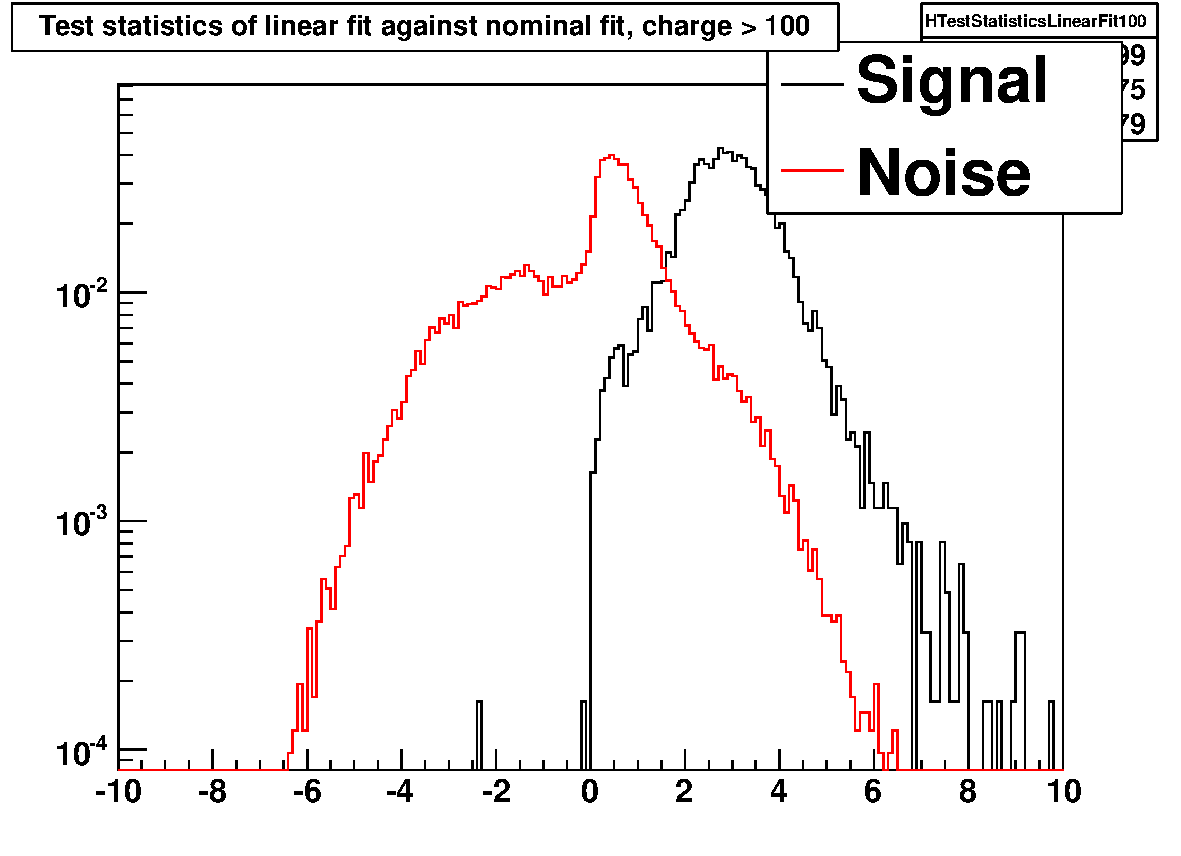
\includegraphics[width=120mm]{DailyLog/6311/6311HTestStatisticsLinearFit100.pdf}
\caption{Test statistics on linear fit, charge \textgreater 100 fC.}
\label{Figure_6311HTestStatisticsLinearFit100}
\end{figure}

\DailySection{Vecbos candle note}

Let's form the items that need to be written here...

\begin{enumerate}
\item Introduction
\item Data \& MC samples
\item ECAL spike cleaning
\item Jet flavors.
\item Selections.  Muon, Z.  Isolation
\item Signal extraction (fit strategy)
\item Toy studies: shape, parameters
\item Toy studies: show that the errors are reasonable (!)
\item JES uncertainty
\item Anti-muon control sample
\end{enumerate}

\DailySection{Installing (temporary) Hcal DQM GUI on lxplus}

Following instructions on \url{https://twiki.cern.ch/twiki/bin/view/CMS/DQMTest}....and the DQM GUI is there. \texttt{=\_\_\_+}

After starting the GUI and the collector, run on \texttt{hcal\_dqm\_sourceclient-file\_cfg.py} (with a few parameters changed).
While the job is running, the GUI responds and I can see the plots.  But once it's done running, the DQM plots are not there anymore....

Now I should ask what Artur wants to be done for the DQM.

As a start, the following can be done relatively quickly according to Artur:

\begin{enumerate}
\item Understand the basic histograms (especially the ones in the summary page)
\item Adding code from Shuichi
\item Check if there is any other useful parameters that could be incorporated into the DQM.
\end{enumerate}

\DailySection{Reflection}

\DailySection{Goals for next work day}

\begin{enumerate}
\item Write Z candle note - have all the individual paragraphs ready by end of Wednesday!
\item Read Hcal DQM code
\item Double-spike....?
\item Setup script that takes the output of the Z candle fit and calculate ratio
\end{enumerate}


